\documentclass[a4paper,11.5pt]{article}
\usepackage[textwidth=170mm, textheight=230mm, inner=20mm, top=20mm, bottom=30mm]{geometry}
\usepackage[normalem]{ulem}
\usepackage[utf8]{inputenc}
\usepackage[T1]{fontenc}
\PassOptionsToPackage{defaults=hu-min}{magyar.ldf}
\usepackage{pgfplots}
\pgfplotsset{compat=1.10}
\usepgfplotslibrary{fillbetween}
\usepackage[magyar]{babel}
\usepackage{amsmath, amsthm,amssymb,paralist,array, ellipsis, graphicx, float, bigints,tikz}
%\usepackage{marvosym}

\makeatletter
\renewcommand*{\mathellipsis}{%
	\mathinner{%
		\kern\ellipsisbeforegap%
		{\ldotp}\kern\ellipsisgap
		{\ldotp}\kern\ellipsisgap%
		{\ldotp}\kern\ellipsisaftergap%
	}%
}
\renewcommand*{\dotsb@}{%
	\mathinner{%
		\kern\ellipsisbeforegap%
		{\cdotp}\kern\ellipsisgap%
		{\cdotp}\kern\ellipsisgap%
		{\cdotp}\kern\ellipsisaftergap%
	}%
}
\renewcommand*{\@cdots}{%
	\mathinner{%
		\kern\ellipsisbeforegap%
		{\cdotp}\kern\ellipsisgap%
		{\cdotp}\kern\ellipsisgap%
		{\cdotp}\kern\ellipsisaftergap%
	}%
}
\renewcommand*{\ellipsis@default}{%
	\ellipsis@before
	\kern\ellipsisbeforegap
	.\kern\ellipsisgap
	.\kern\ellipsisgap
	.\kern\ellipsisgap
	\ellipsis@after\relax}
\renewcommand*{\ellipsis@centered}{%
	\ellipsis@before
	\kern\ellipsisbeforegap
	.\kern\ellipsisgap
	.\kern\ellipsisgap
	.\kern\ellipsisaftergap
	\ellipsis@after\relax}
\AtBeginDocument{%
	\DeclareRobustCommand*{\dots}{%
		\ifmmode\@xp\mdots@\else\@xp\textellipsis\fi}}
\def\ellipsisgap{.1em}
\def\ellipsisbeforegap{.05em}
\def\ellipsisaftergap{.05em}
\makeatother

\usepackage{hyperref}
\hypersetup{
	colorlinks = true	
}

\DeclareMathOperator{\Int}{int}
\DeclareMathOperator{\tg}{tg}
\DeclareMathOperator{\ctg}{ctg}
\DeclareMathOperator{\Th}{th}
\DeclareMathOperator{\sh}{sh}
\DeclareMathOperator{\ch}{ch}
\DeclareMathOperator{\arsh}{arsh}
\DeclareMathOperator{\arch}{arch}
\DeclareMathOperator{\arth}{arth}
\DeclareMathOperator{\arcth}{arcth}
\DeclareMathOperator{\grad}{grad}
\DeclareMathOperator{\arc}{arc}
\DeclareMathOperator{\arctg}{arc tg}
\DeclareMathOperator{\arcctg}{arc ctg}
\newcommand{\norm}[1]{\left\lVert#1\right\rVert}

\begin{document}
	%%%%%%%%%%%RÖVIDÍTÉSEK%%%%%%%%%%
	\setlength\parindent{0pt}
	\def\a{\textbf{a}}
	\def\b{\textbf{b}}
	\def\N{\hskip 10 true mm}
	\def\a{\textbf{a}}
	\def\b{\textbf{b}}
	\def\c{\textbf{c}}
	\def\d{\textbf{d}}
	\def\e{\textbf{e}}
	\def\gg{$\gamma$}
	\def\vi{\textbf{i}}
	\def\jj{\textbf{j}}
	\def\kk{\textbf{k}}
	\def\fh{\overrightarrow}
	\def\l{\lambda}
	\def\m{\mu}
	\def\v{\textbf{v}}
	\def\0{\textbf{0}}
	\def\s{\hspace{0.2mm}\vphantom{\beta}}
	\def\Z{\mathbb{Z}}
	\def\Q{\mathbb{Q}}
	\def\R{\mathbb{R}}
	\def\C{\mathbb{C}}
	\def\N{\mathbb{N}}
	\def\Rn{\mathbb{R}^{n}}
	\def\Ra{\overline{\mathbb{R}}}
	\def\sume{\displaystyle\sum_{n=1}^{+\infty}}
	\def\sumn{\displaystyle\sum_{n=0}^{+\infty}}
	\def\biz{\emph{Bizonyítás:\ }}
	\def\narrow{\underset{n\rightarrow+\infty}{\longrightarrow}}
	\def\limn{\displaystyle\lim_{n\to +\infty}}
	%	\def\definition{\textbf{Definíció:\ }}
	%	\def\theorem{\textbf{Tétel:\ }}
	%\def\note{\emph{Megjegyzés:\ }}
	%\def\example{\textbf{Példa:\ }} 
	
	\theoremstyle{definition}
	\newtheorem{theorem}{Tétel}[subsubsection] % reset theorem numbering for each chapter
	
	\theoremstyle{definition}
	\newtheorem{definition}[theorem]{Definíció} % definition numbers are dependent on theorem numbers
	\newtheorem{example}[theorem]{Példa} % same for example numbers
	\newtheorem{exercise}[theorem]{Házi feladat} % same for example numbers
	\newtheorem{note}[theorem]{Megjegyzés} % same for example numbers
	\newtheorem{task}[theorem]{Feladat} % same for example numbers
	\newtheorem{revision}[theorem]{Emlékeztető} % same for example numbers
	%%%%%%%%%%%%%%%%%%%%%%%%%%%%%%%%%
	\begin{center}
		{\LARGE\textbf{Analízis 3. A szakirány}}
		\smallskip
		
		{\Large Gyakorlati jegyzet}
		
		\smallskip
		11. óra.
	\end{center}
	A jegyzetet \textsc{Umann} Kristóf készítette \textsc{Filipp} Zoltán István gyakorlatán. (\today)
	%\subsection{Taylor-polinomok folytatása}
	
	\begin{task}
		\[ f(x,y)=x^y+y^2\cdot\cos(x-1)\quad (x,y)\in\R^2,\quad x>0 \]
		Tekintsük az $a=(1,3)$ pontot és számítsuk ki $T_2f(x,y)$-t!
		
		\textit{Megoldás:} 
		\[ T_2f(x,y)=\overbrace{f(1,3)}^{k=0}+\overbrace{\partial_1f(1,3)(x-1)+\partial_2f(1,3)(y-3)}^{k=1}+\frac{1}{2}\partial_{11}f(1,3)\cdot(x-1)^2+\partial_{12}f(1,3)(x-1)(y-3)+\frac{1}{2}\partial_{22}f(1,3)(y-3)^2 \]
		\[ f(1,3)=1^3+9\cos0=10 \]
		Ekkor:
		\begin{align*}
			\partial_1f(x,y)=&\ y\cdot x^{y-1} + y^2\cdot(-\sin(x-1))\cdot1=y\cdot x^{y-1}-y^2\cdot\sin(x-1)\\
			\partial_2f(x,y)=&\ x^y\cdot\ln x+2y\cdot\cos(x-1)\\
			\partial_{11}f(x,y)=&\ y(y-1)x^{y-2}-y^2\cos(x-1)\\
			\partial_{12}f(x,y)=&\ y\cdot x^{y-1}\ln x + x^y\cdot\frac{1}{x}-2y\cdot\sin(x-y)=\partial_{21}f(x,y)\\
			\partial_{22}f(x,y)=&\ x^y(\ln x)^2 +2\cos(x-1)
		\end{align*}
		Így:
		\begin{align*}
			\partial_1f(x,y)=&\ 3\\
			\partial_2f(x,y)=&\ 6\\
			\partial_{11}f(x,y)=&\ 6-9=-3\\
			\partial_{12}f(x,y)=&\ 1\\
			\partial_{22}f(x,y)=&\ 2
		\end{align*}
		Ez alapján
		\[ T_2f(x,y)=10+3(x-1)+6(y-3)-\frac{3}{2}(x-1)^2+(x-1)(y-3)+(y-3)^2 \quad \big((x,y)\in\R^2\big) \]
	\end{task}
	\begin{note}\
		\[ T_1f(x,y)=10+3(x-1)+6(y-3)\quad \big((x,y)\in\R^2\big) \]
		Ez az érintő sík függvénye lesz az $(1,3)$-nak, vagy másképp:
		\[ z=10+3(x-1)+6(y-3)\quad \Leftrightarrow\quad  3x+6y-z=11. \]
		Ez utóbbi a legegyszerűbb alakja az érintő sík egyenletének.
	\end{note}
	\begin{note}
		ZH-ban maximum egy harmadrendű polinom várható, és le se kell vezetni multiindexekkel.
	\end{note}
	\begin{note}
		A formula felírása 1 pont, a deriváltak felírása szintén (darabonként), a megoldás felírása 1 pont (nem darabonként).
	\end{note}
	\begin{exercise}
		Adjuk meg a
		\[ f(x,y)=\sqrt{x^2+2y^2+3xy}\quad \big((x,y)\in(0,+\infty)\big) \]
		függvénynek az $a=(1,2)$ pontban az érintő síkjának egyenletét. (ez az elsőfokú Taylor polinom)
	\end{exercise}
	\begin{note}
		\[ f(a+h)=f(a)+\langle f'(a); h\rangle + \frac{1}{2}\langle f''(a)\cdot h, h\rangle+\nu(h)\cdot\norm{h}^2 \]
		ahol:
		\[ f\in\R^n\to\R;\quad f'(a)=\big(\partial_1 f(a),\ldots,\partial_nf(a) \big);\quad \left[ a+h=(x,y),\quad h=(x,y)-a\right] \]
		És a Hesse mátrix:
		\[
			\begin{bmatrix}
				\partial_{11}f(a)&\dots&\partial{n1}f(a)\\
				\partial_{12}f(a)&\dots&\partial{n2}f(a)\\
				\vdots&&\vdots\\
				\partial_{1n}f(a)&\dots&\partial{nn}f(a)
			\end{bmatrix} = \left[\partial_{ij}f(a) \right]^n_{i,j=1}
		\]
	\end{note}
	\subsection{Lokális szélső érték keresés}
	\begin{example}
		\[ f(x,y)=x^2+xy+y^2-5x-4y+1\quad \big((x,y)\in\R^2\big) \]
		lokális szélső érték = ?
		
		\textit{Megoldás:} Első lépésben határozzuk meg a parciális deriváltakat.
		\begin{align*}
			\partial_1f(x,y)&=2x+y-5 = 0\\
			\partial_2f(x,y)&=x+2y-4=0\\
		\end{align*}
		Ezt az egyenletrendszert oldjuk meg, így $x=2, y=1$. Stacionárius hely a $(2,1)$ pont, itt \textbf{lehet} lokális szélső értéke $f$-nek (mivel $f\in D(\R^2)$, hisz pl. $\exists \partial_1f,\partial_2f\in C(\R^2)$, így az összes lehetséges szélsőértékhely meglesz az $f'=0$ rendszerből.
		
		Második lépésben: 
		\begin{align*}
			\partial_{11}f(x,y)&=2 \\
			\partial_{12}f(x,y)&=1 \\
			\partial_{22}f(x,y)&=2 
		\end{align*} 
		$\forall(x,y)\in\R^2$ spec. $(2,1)$-ben is.
		\[ \Rightarrow\quad f(x,y)=\begin{bmatrix}
			2&1\\
			1&2
		\end{bmatrix}\quad \Rightarrow\quad f''(2,1)\begin{bmatrix}
			2&1\\
			1&2
		\end{bmatrix}\quad \Leftrightarrow\quad \varDelta_1=2>0,\quad \varDelta_2=3>0 \]
		Ahol $\varDelta_i$ az $i$-edik főminor. Mivel így ez a mátrix pozitív definit, a Sylvester tételből így következik, hogy $f''(2,1)$ lokális minimum hely, értéke $f(2,1)=6$
		%TODO 01
		\begin{figure}[H]
			\centering
			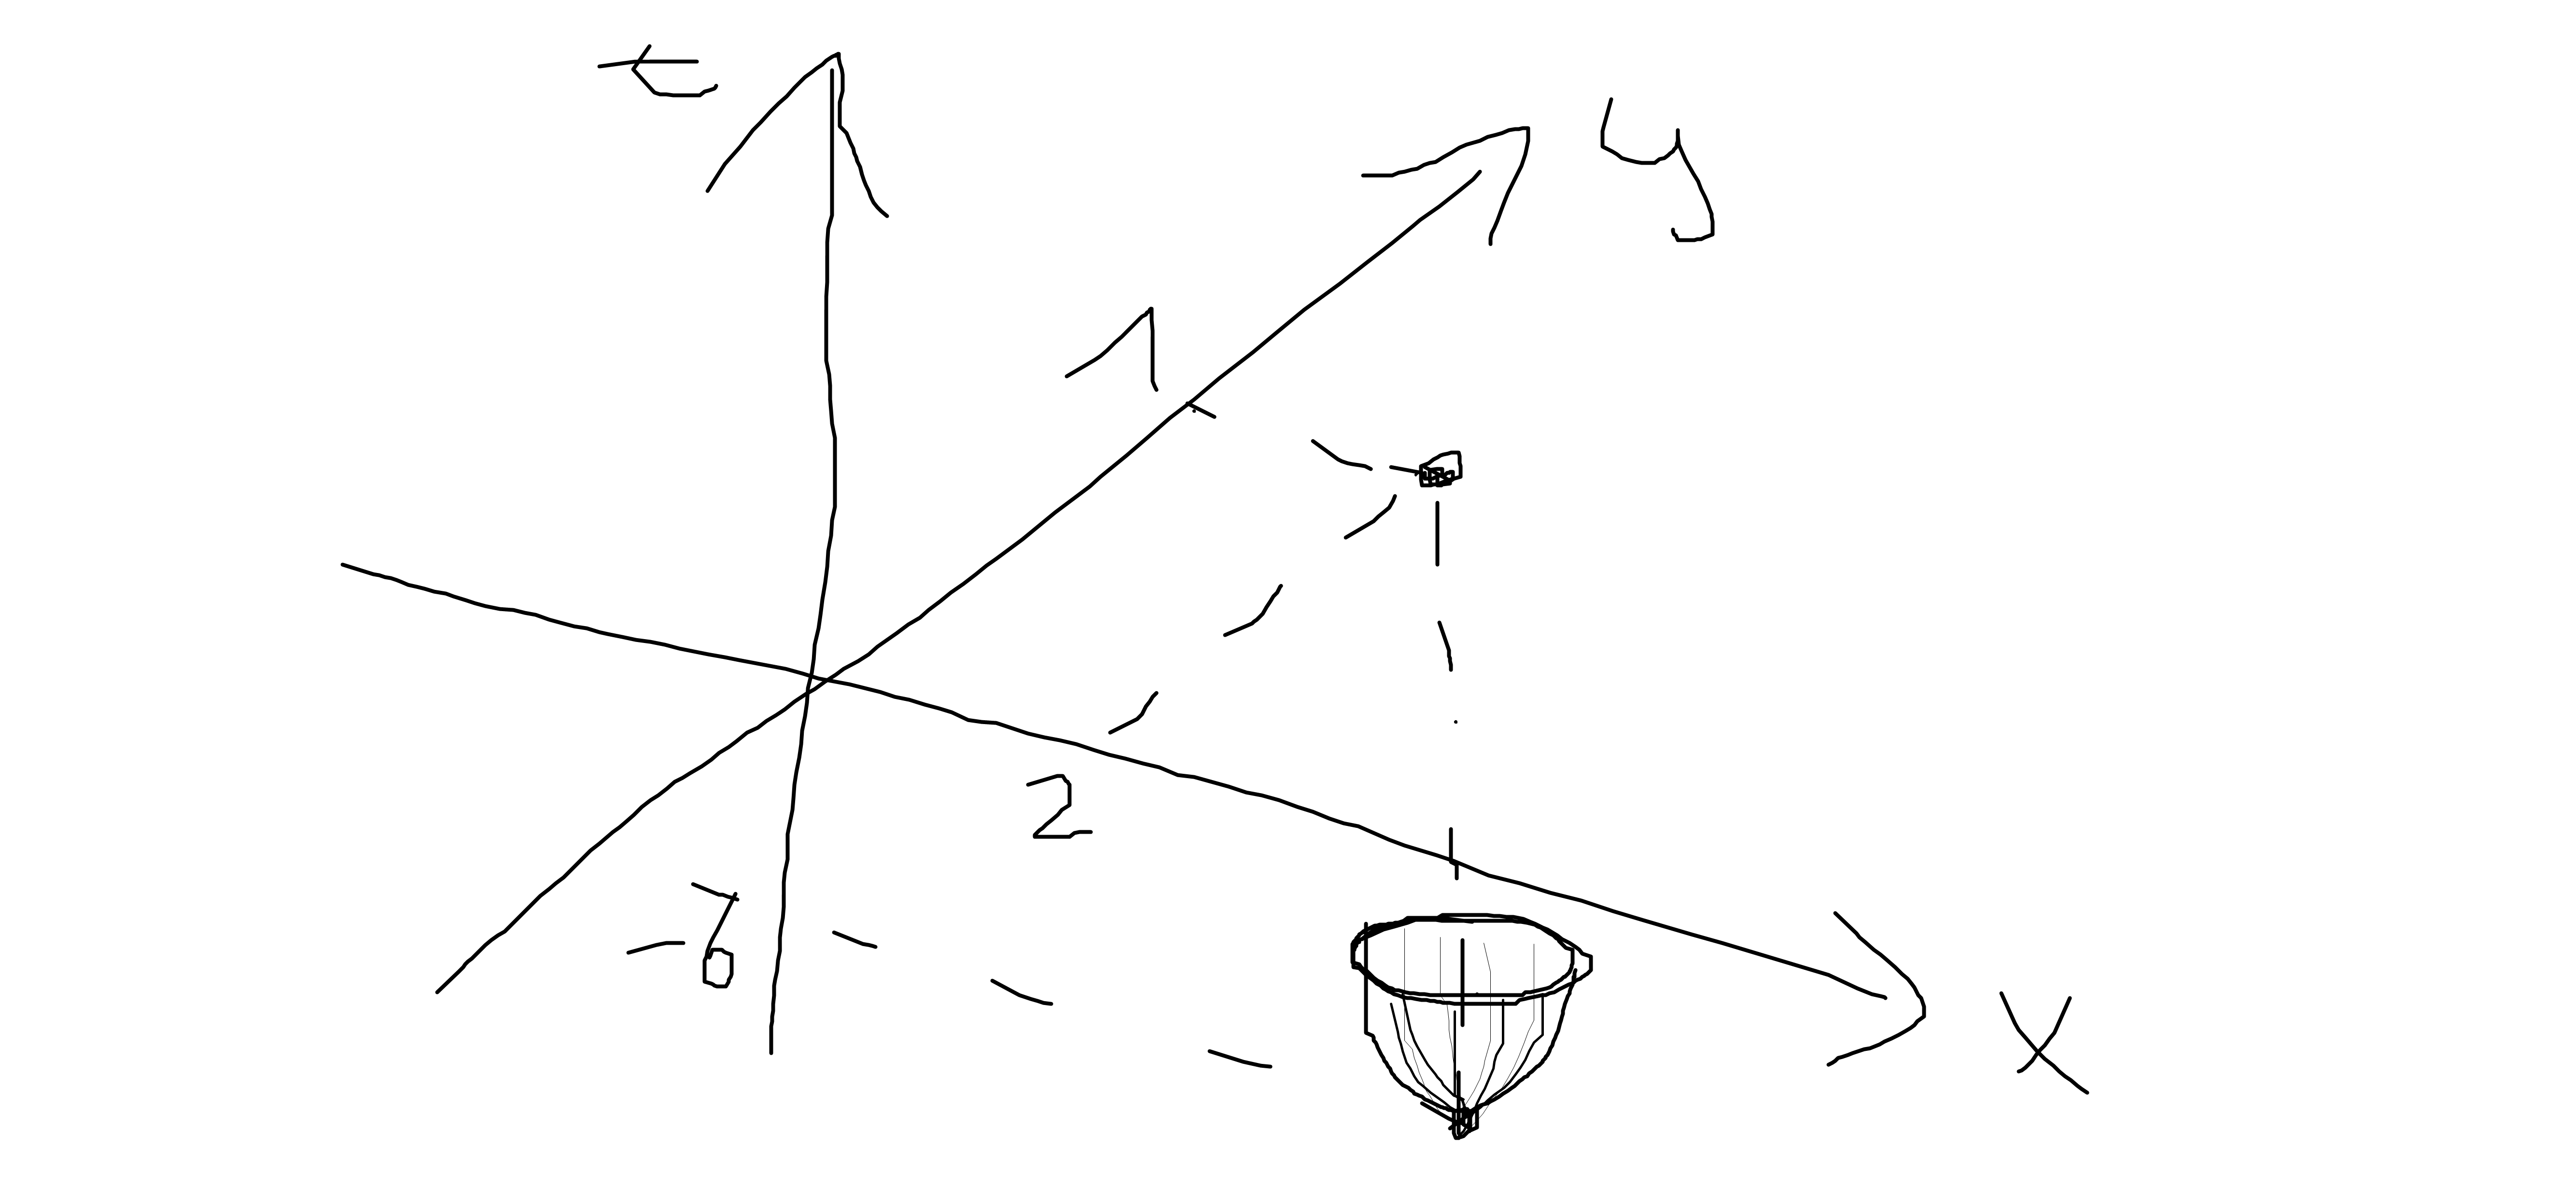
\includegraphics[height=4cm]{kepek/38.png}
			\caption{}
		\end{figure}
	\end{example}
	\begin{task}
		\[ f(x,y)=(1+e^y)\cos x-y\cdot 3^y\quad \big((x,y)\in\R^2 \big) \]
		Keressük meg a lkális szélső érték(ek)et.
		
		\textit{Megoldás:} Első lépés:
		\[\left.\begin{gathered}
			\partial_1f(x,y)=(1+e^y)(-\sin x)=0\\
			\partial_2f(x,y)=e^y\cdot\cos x-e^y-y\cdot e^y=0\\
		\end{gathered}\right\}  \]
		Ez alapján
		\[\begin{cases}
			\sin x=0\quad \Leftrightarrow\quad X_k=k\pi\quad (k\in\Z)\\
			\cos x-1-y=0\quad \Leftrightarrow\quad y_k=\cos(k\pi)-1=(-1)^k-1
		\end{cases}\]
		Ez alapján a stacionárius helyek: $\big((k\pi; (-1)^k-1)\quad k\in\Z\big)$, azaz
		\[ (2k\pi,0)\quad \text{és}\quad ((2k+1)\pi; -2) \quad (k\in\Z)\]
		\begin{figure}[H]
			\centering
			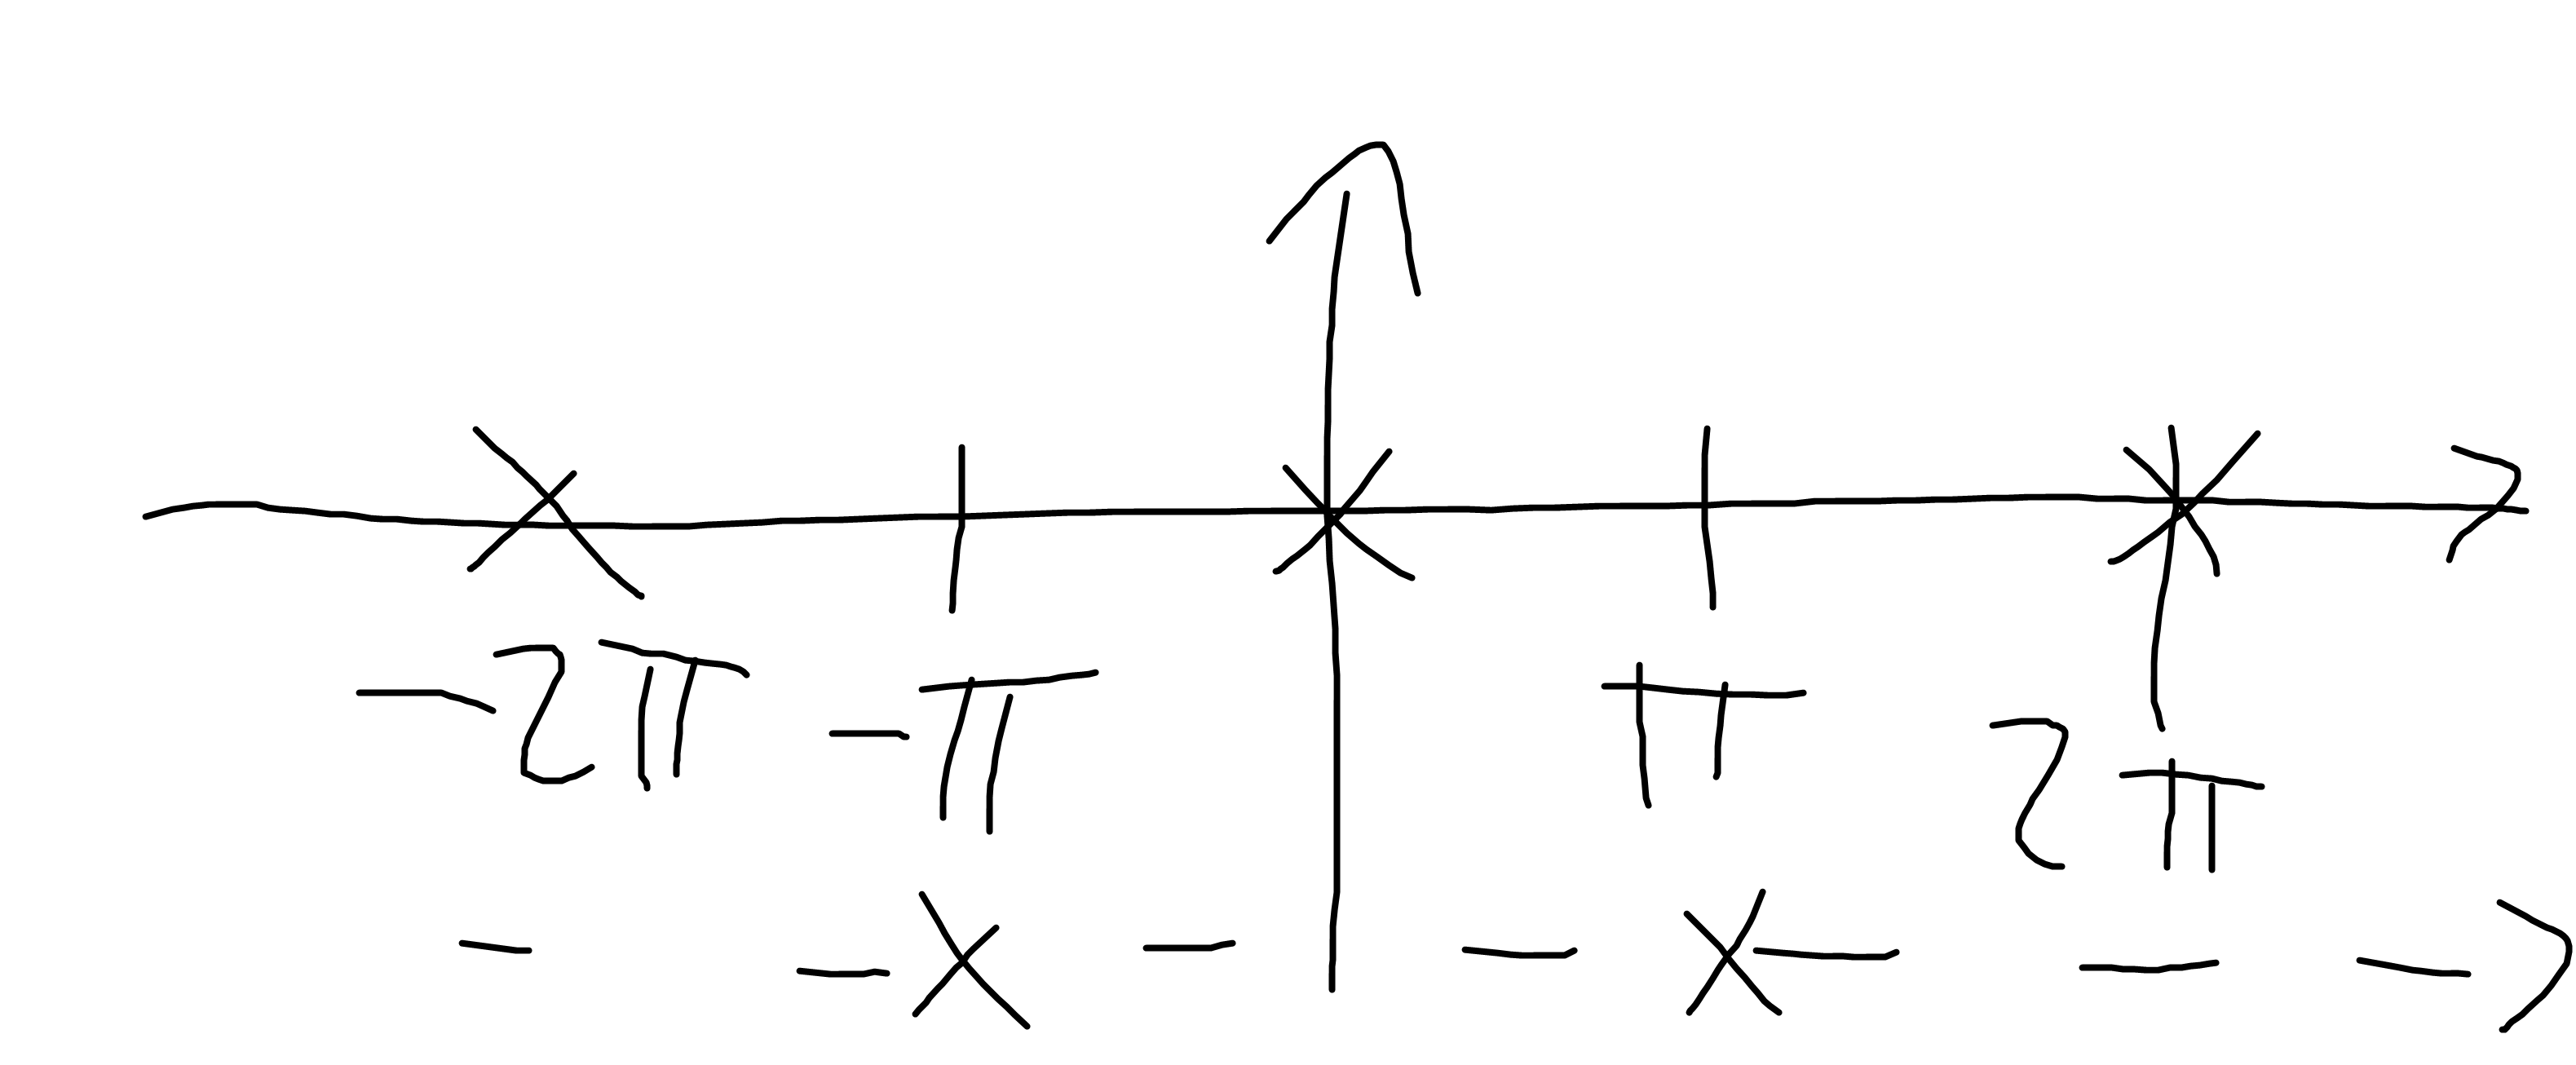
\includegraphics[height=4cm]{kepek/39.png}
			\caption{}
		\end{figure}
		Második lépés
		\begin{align*}
			\partial_{11}f(x,y)=-(1+e^y)\cos x\\
			\partial_{12}f(x,y)=-e^y\sin x\\
			\partial_{22}f(x,y)=e^y\cos x-e^y-e^y-ye^y
		\end{align*}
		\[ \Rightarrow\quad f''(x,y)=\begin{bmatrix}
			-(1+e^y)\cos x&-e^y\sin x\\
			-e^y\sin x&e^y\cos x-2e^y-ye^y
		\end{bmatrix}\quad \Rightarrow\quad \overbrace{f''(2k\pi,0)}^{k\in\Z}=\begin{bmatrix}
			-2&0\\
			0&-1
		\end{bmatrix},\quad \varDelta_1=-2>0, \quad \varDelta_2=2>0 \]
		Ez a Sylvester tétel szerint $f''(2k\pi,0)$ egy negatív definit mátrix$\quad \Rightarrow\quad \forall k\in\Z \quad (2k\pi,0)$ pontok lokális maximum helyek. Értékük: $(2k\pi,0)=(1+e^0)\cos2k\pi=2$.
		
		Illetve:
		\[f''((2k+1)\pi;-2)=\begin{bmatrix}
			1+\frac{1}{e^2}&0\\
			0&-\frac{1}{e^2}
		\end{bmatrix},\quad \varDelta_1=1+\frac{1}{e^2}>0,\quad \varDelta_2=-\frac{1}{e^2}<0 \]
		$\Rightarrow\quad f''((2k+1)\pi,2)\quad (\forall k\in\Z)$ indefinit mátrix. A másodrendű szükséges feltétel alapján ezek $((2k+1)\pi,2)\quad (k\in\Z)$ biztosan nem lokális szélső érték helyek (NYEREG PONTOK).
	\end{task}
	\begin{task}
		\[ f(x,y)=x^4+y^4-x^2-2xy-y^2\quad \big((x,y)\in\R^2\big) \]
		\textit{Megoldás:}
		\begin{align*}
			\partial_1f(x,y)=4x^3-2x-2y=0\\
			\partial_2f(x,y)=4y^3-2x-2y=0\\
		\end{align*}
		\[ 4x^3-4y^3=0\quad \Leftrightarrow\quad x^3=y^3\quad \Leftrightarrow\quad x=y \]
		\[ 4x^3-4x=0\quad \Leftrightarrow\quad 4x(x^2-1)=0 \]
		Ez alapján
		\begin{align*}
			x_1=y_1=0\\
			x_2=y_2=1\\
			x_3=y_3=-1\\
		\end{align*}
		Stacionárius helyek: $(0,0),\quad (1,1),\quad (-1,-1)$
		\begin{figure}[H]
			\centering
			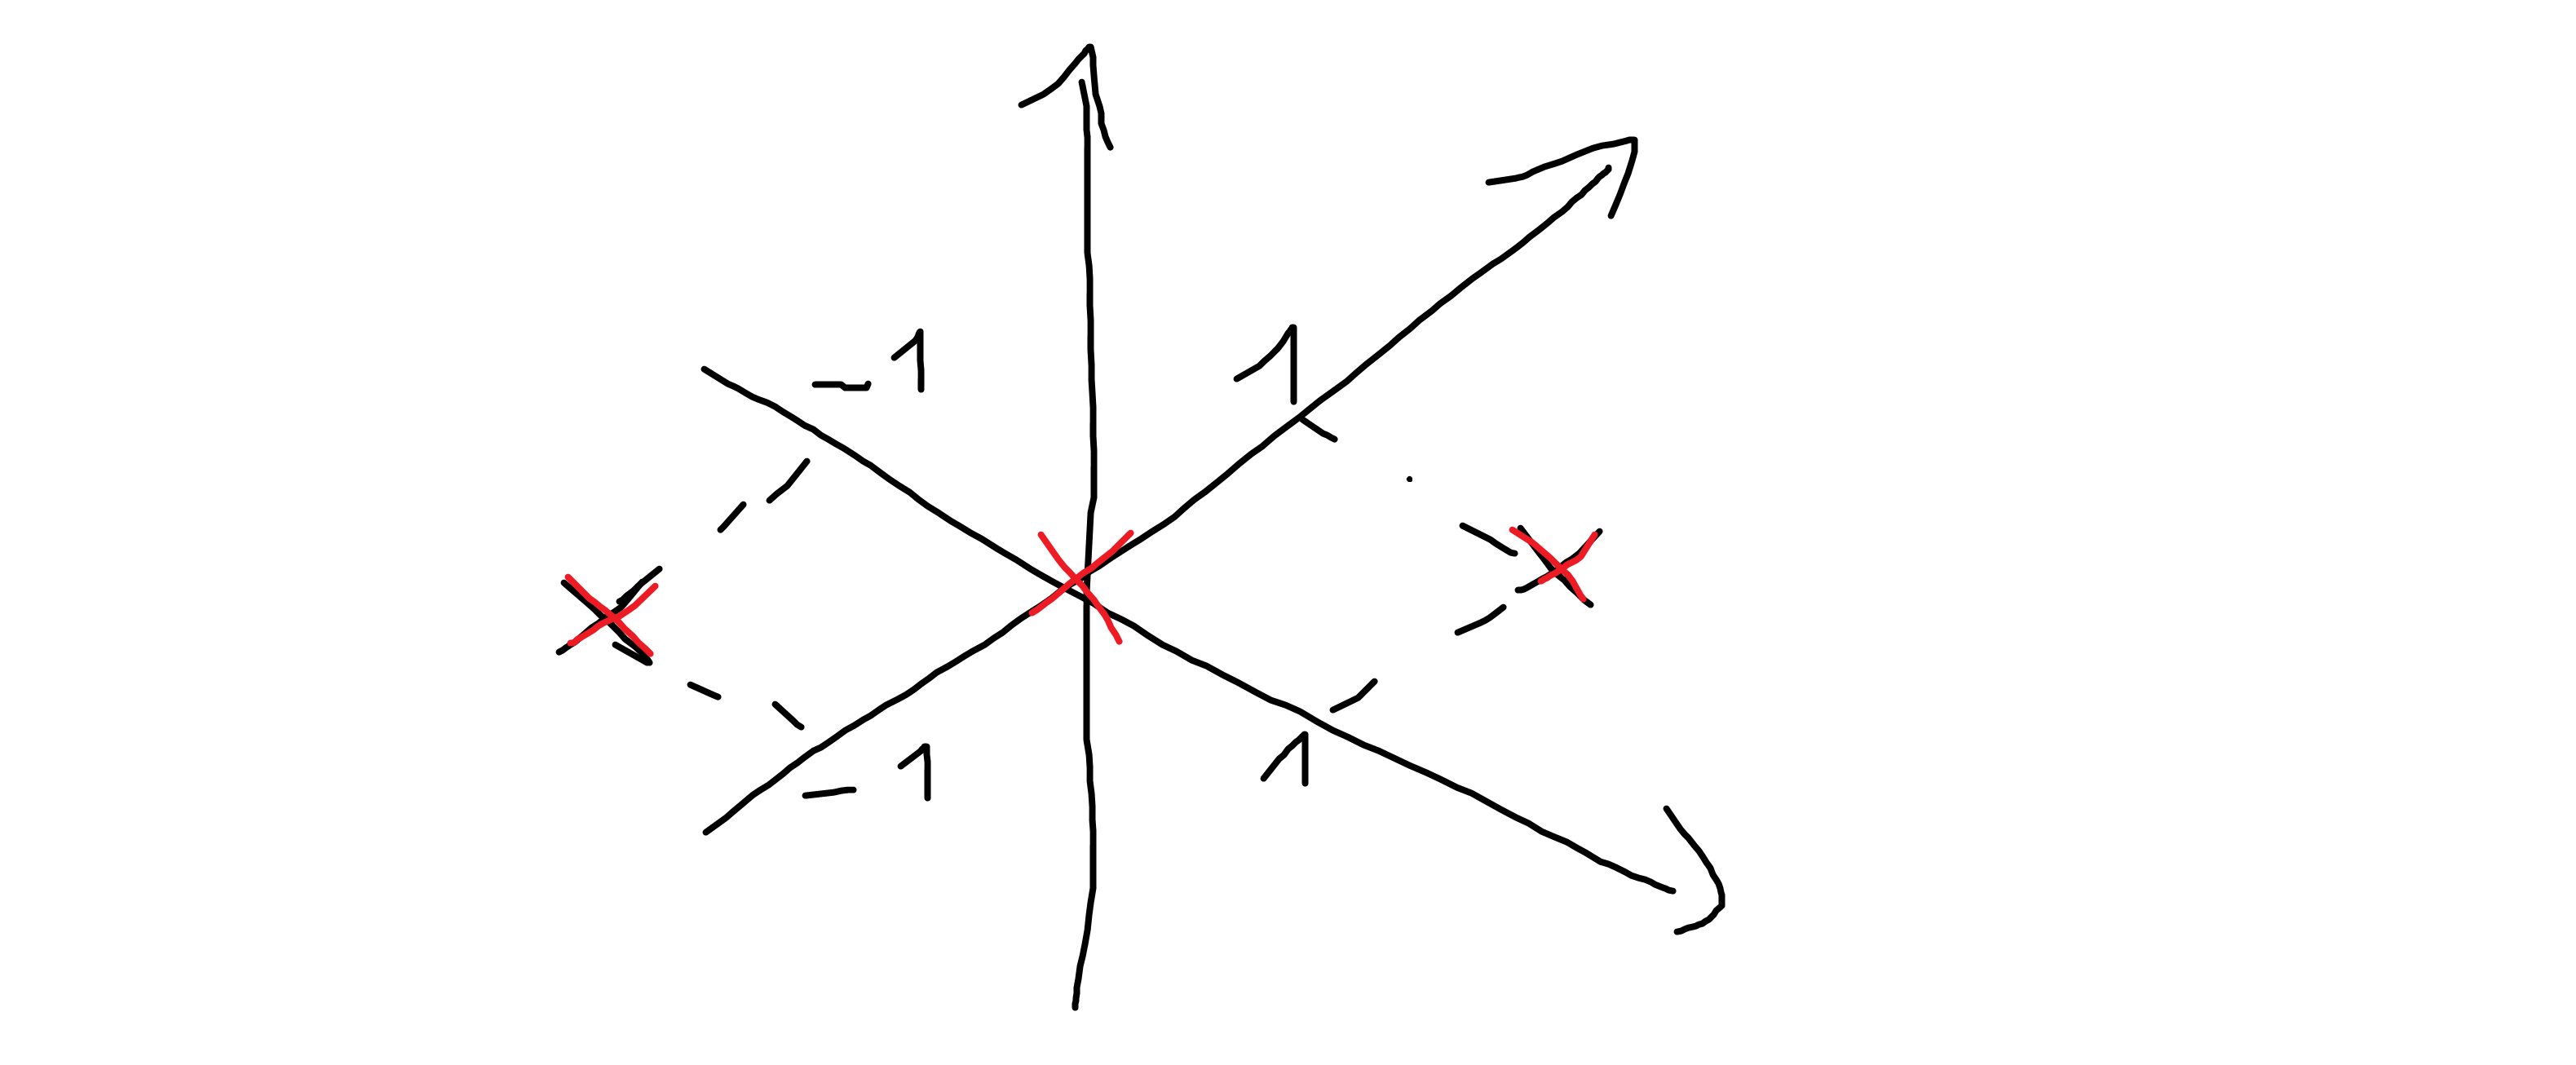
\includegraphics[height=4cm]{kepek/40.png}
			\caption{}
		\end{figure}
		\begin{align*}
			\partial_{11}f(x,y)=12x^2-2
			\partial_{12}f(x,y)=-2
			\partial_{22}f(x,y)=12y^2-2
		\end{align*}
		A Hesse mátrix ez alapján
		\[ f''(x,y)=\begin{bmatrix}
			12x^2-2&-2\\
			-2&12y^2-2
		\end{bmatrix} \]
		Először vizsgáljuk meg az (1,1) helyen:
		\[ f''(1,1)=\begin{bmatrix}
			10&-2\\
			-2&10
		\end{bmatrix}\quad \delta_1=10>0,\quad \delta_2=96>0 \] 
		Pozitív definit mátrixok $\quad \Rightarrow\quad (1,1)$ és $(-1,-1)$ is minimum helyek, értékük $f(1,1)=f(-1,-1)=-2$
		
		Most tekintsük a (0,0) helyet:
		\[ f''(0,0)=\begin{bmatrix}
			-2&-2\\
			-2&-2
		\end{bmatrix}\quad \delta_1=2>0,\quad \delta_2=0 \]
		Negatív szemidefinit, itt msot nem alkalmazhatjuk a tételt, további vizsgálat kell.
		\begin{center}
			[gondolatmenet közepe]
			\smallskip
			
			\textit{,,Ha valakinek a nevében P betű van, az a tanítást és igehirdetést jelenti.''}
			
			/Filipp/
			\medskip
			
			\textit{,,Illés Zoltán''}
			
			/Husi/
		\end{center}
	\end{task}
\end{document}